\section{Rauschen in analogen Kommunikationssystemen \formelbuch{202-8}}
\textbf{Rauschen} \textbf{verschlechtert} die \textbf{Performance}. Bei \textbf{analogen} Systemen
macht sich dies beim \textbf{Signal-Rausch-Abstand (SNR)} bemerkbar.
\begin{figure}[!ht]
\begin{center}
	\begin{tikzpicture}[>=latex']
    \node[input, name=input] {};
    \node[block, right of=input, name=transmitter] {Transmitter};
    \node[block, right of=transmitter, name=channel, node distance=3cm] {Channel};
    \node[sum, right of=channel, name=sum, pin={[pin style]above:$n(t)$}] {$\Sigma$};
    \node[block, right of=sum, name=receiver] {Receiver}; 
    \node[output, right of=receiver, name=output, node distance=2cm] {};        
    
    \draw[->] (input) -- (transmitter)
       node[above, near start] (Xt) {$X(t)$}
       node[below, near start] (Xt) {$S_x$};
    \draw[->] (transmitter) -- node[below] {$S_t$} (channel);
    \draw[->] (channel) -- (sum);
    \draw[->] (sum) -- (receiver)
       node[above, midway] {$Y_i(t)$}
       node[below, midway] {$S_i, N_i$};
    \draw[->] (receiver) -- (output)
       node[above, near end] {$Y_o(t)$}
       node[below, near end] {$S_o, N_o$};
\end{tikzpicture}    
\end{center}
\end{figure}
Die Voraussetzungen für eine einfache Berechnung mit Hilfe von diesem Modell (gauss'scher Kanal)
sind die folgenden:
\begin{itemize}
  \item $n(t)$ ist \textbf{mittelwertfreies} ($E[n] = 0$) gauss'sches Rauschen mit ..
  \item $S_{nn}(\omega) = \eta/2$ und $\ldots$
  \item ist mit $X \left( t \right)$ \textbf{unkorreliert} $\left( \cov
  \left(X,n \right) = E \left[ X \cdot n \right] - E \left[ X \right] \cdot E
  \left[ n \right] = 0 \right)$
\end{itemize}
Somit gilt: $\qquad E[(X_0 + n_0)^2] = E[X_0^2] + E[2 \cdot X_0 \cdot n_0] + E[n_0^2] = S_0 + N_0
\qquad \text{ und } \qquad \left(\dfrac{S}{N}\right)_0 = \dfrac{E[X_0(t)^2]}{E[n_0(t)^2]}$ \\ \\
Weist der Kanal eine \textbf{Dämpfung} $A_{db}$ auf, so muss diese bei den Berechnungen berücksichtigt
werden: $S_{i_{dB}} = S_{t_{dB}} - A_{dB}$



\skriptsubsection{Basisband}{203-8.3}
Die Berechnungen im Basisband gelten als \textbf{Referenz}, für den \textbf{Vergleich} mit
\textbf{anderen Systemen}. \\
\begin{figure}[!ht]
\begin{center}
	\begin{tikzpicture}[>=latex']
    \node[input, name=input] {};
    \node[block, right of=input, name=lpf1, node distance=2cm] {LPF};
    \node[block, right of=lpf1, name=channel, node distance=2.8cm] {Channel};
    \node[sum, right of=channel, name=sum, pin={[pin style]above:$n(t)$}, node distance = 2cm] {$\Sigma$};
    \node[block, right of=sum, name=lpf2] {LPF}; 
    \node[output, right of=lpf2, name=output, node distance=2cm] {};        
    
    \draw[->] (input) -- (lpf1)
       node[above, near start] {$X(t)$}
       node[below, near start] {$S_x$} ;
    \draw[->] (lpf1) -- node[below] {$S_t$} (channel);
    \draw[->] (channel) -- (sum);
    \draw[->] (sum) -- (lpf2)
       node[above, midway] {$Y_i(t)$}
       node[below, midway] {$S_i, N_i$};
    \draw[->] (lpf2) -- (output)
       node[above, near end] {$Y_0(t)$}
       node[below, near end] {$S_0, N_0$};
\end{tikzpicture}
\end{center}
\end{figure}
Wiederum müssen wieder gewisse Einschränkungen gemacht werden für eine einfachere Berechnung:
\begin{itemize}
  \item $X(t)$ ist mittelwertfrei $\quad \Rightarrow \quad E[X]=0$
  \item $X(t)$ ist stationär und ergodisch $\quad \Rightarrow \quad <x_{\lambda}(t)> = E[X] = 0
  \quad (\text{für alle } x_{\lambda}(t))$
  \item $X(t)$ ist bandbeschränkt ($S_{XX}(\omega) = 0 $ für $\omega > W$) durch den Tiefpasfilter
  mit idealer Bandbreite $W = 2 \pi B$
  \item Der Kanal ist verzerrungsfrei
\end{itemize}

$$ \text{Die Rauschleistung im Basisband: } \qquad \boxed{\left(\dfrac{S}{N}\right)_0 =
\dfrac{S_0}{N_0} = \dfrac{S_i}{\eta B} = \gamma} \qquad \text{dient zum Vergleich mit anderen
Systemen.}$$

\skriptsubsection{Amplitudenmodulation}{204-8.4}
\begin{figure}[!ht]
\begin{center}
	\begin{tikzpicture}[>=latex']
    \node[input, name=input] {};
    \node[block, right of=input, name=transmitter, node distance=2.2cm, text width=6em] {Transmitter (modulator)};
    \node[block, right of=transmitter, name=channel, node distance=3.2cm] {Channel};
    \node[sum, right of=channel, name=sum, pin={[pin style]above:$n(t)$}, node distance = 2cm] {$\Sigma$};
    \node[block, right of=sum, name=bpf, node distance = 2cm] {BPF};
    \node[block, right of=bpf, name=detector, node distance=3.4cm] {Detector};
    \node[block, right of=detector, name=lpf] {LPF};
    \node[output, right of=lpf, name=output, node distance=2.4cm] {};        
    
    \draw[->] (input) -- (transmitter)
       node[above, near start] {$X(t)$}
       node[below, near start] {$S_x$} ;
    \draw[->] (transmitter) -- node[above] {$X_c(t)$} (channel);
    \draw[->] (channel) -- (sum);
    \draw[->] (sum) -- (bpf);
    \draw[->] (bpf) -- node[above, near start] {$Y_i(t)$} (detector);
    \draw[->] (detector) -- (lpf);
    \draw[->] (lpf) -- (output)
       node[above, near end] {$Y_0(t)$};
    
    %% Rechtecke
    \node at ($(detector.south west)-(0.3cm,0.4cm)$) (demo_SW) {};
    \node at ($(lpf.north east)+(0,0.1cm)$) (demo_NE) {};
    \node[draw=black, rectangle, dashed, fit=(demo_SW) (demo_NE)] (demodulator) {};
    \node[anchor=south east] at (demodulator.south east) {Demodulator};
    
    \node at ($(bpf.south west)-(0.2cm,0.8cm)$) (rec_SW) {};
    \node at ($(lpf.north east)+(0.3cm,0.4cm)$) (rec_NE) {};
    \node[draw=black, rectangle, dashed, fit=(rec_SW) (rec_NE)] (receiver) {};
    \node[anchor=south west] at (receiver.south west) {Receiver};
\end{tikzpicture}
\end{center}
\end{figure}
Das Rauschsignal am Eingang des Demodulators ist wie folgt definiert
\verweis{schmalbandiger_zufallsprozess}{Schmalbandiger Zufallsprozess}:  
$$n_i(t) = n_c(t) \cos(\omega_c t) - n_s(t) \sin(\omega_c t) $$


\skriptsubsubsection{DSB-SC, SSB}{205-8.4.A.1,2}
Ein Mass für die Effizienz des Demodulators ist der sogenannte Detektor-Gewinn: \\
$$ \alpha_{d_{DSB-SC}} = \dfrac{\text{SNR}_{out}}{\text{SNR}_{in}} = 2 \approx 3 dB
\qquad \qquad
 \alpha_{d_{SSB}} = \dfrac{\text{SNR}_{out}}{\text{SNR}_{in}} = 1
$$
Ein DSB-SC Demodulator verbessert also die SNR zwischen Ein- und Ausgang um Faktor 2, bei SSB
bleibt die SNR gleich. Da SSB jedoch nur die halbe Bandbreite von DSB-SC besitzt, ist auch die
Eingangs-Rauschleistung bei SSB halb so gross wie bei DSB-SC. \\
Somit haben im Endeffekt SSB und DSB-SC \textbf{dieselbe Rausch-Performance}: 
	$$ \left(\dfrac{S}{N}\right)_0 =
	\dfrac{A_c^2 S_x}{2 \eta B} = \dfrac{\frac12 A_c^2 S_x}{\eta B} = \dfrac{S_i}{\eta B} = \gamma $$

\skriptsubsubsection{Gewöhnliche AM}{206-8.4.A.3}

\textbf{Synchroner Detektor}
$$ \left(\dfrac{S}{N}\right)_0 =
\dfrac{\mu^2 S_x}{1 + \mu^2 S_x} \left(\dfrac{S_i}{\eta B}\right) = \dfrac{\mu^2 S_x}{1 + \mu^2
S_x} \gamma \leq \dfrac{\gamma}{2} \qquad \qquad
\alpha_d = \dfrac{2 \mu^2 S_x}{1 + \mu^2 S_x} \leq 1$$


\textbf{Enveloppe Detektor} \\
Für \boldmath$ \textbf{SNR}_i \gg 1 $ gelten dieselben Formeln wie beim \textbf{synchronen
Detektor}. \\ \\ Für \boldmath$ \textbf{SNR}_i \ll 1 $ lohnt es sich nicht solche
Berechnungen aufzustellen, da das demodulierte Signal \textbf{nicht mehr brauchbar} wird, weil das Rauschen so enorm dominiert. \\
Der \textbf{Übergang} zwischen \textbf{ausreichender} Übertragungsqualität und \textbf{unbrauchbarer}  
Übertragung beginnt ab \unboldmath$ \text{SNR}_{i_{dB}} \approx 10 \text{dB} $ und erfolgt
\textbf{sehr schnell}.

\skriptsubsection{Winkelmodulation}{208-8.5}
\begin{center}
	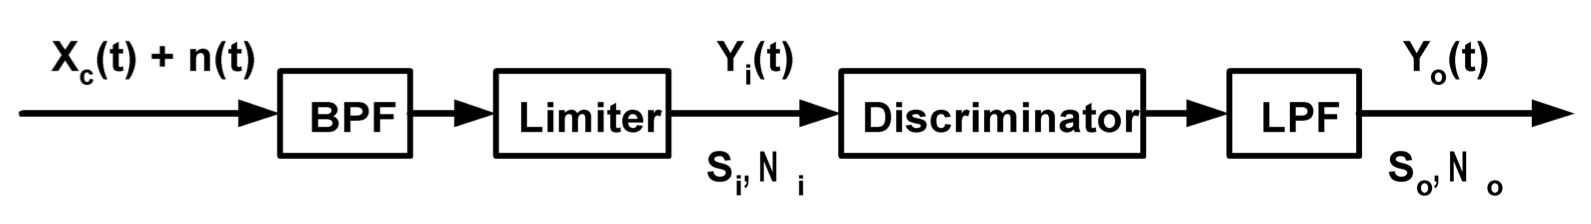
\includegraphics[height=1.3cm]{../NaT2/bilder/08_noise_anglemod.png}
\end{center}
Der Limiter \textbf{limitiert} das Signal - somit auch das Rauschen - in der \textbf{Amplitude}, 
sodass das \textbf{Rauschen} nur noch in der \textbf{Phase enthalten} ist. 
Die \textbf{SNR} wird daher \textbf{nur durch }die \textbf{Phase beeinflusst}. \\ 

Für die Winkelmodulation ist der Träger-Rauschabstand (CNR - Carrier-to-Noise-Ratio) wichtig: 
CNR = $ \dfrac{A_c^2}{2 \eta B_T} = \left(\dfrac{S}{N}\right)_i$. \\
\textbf{Nur wenn} das \textbf{Signal dominant} ist (CNR $\gg 1$), können die unten aufgeführten
Formeln angewendet werden. \\ 
Im Falle von (CNR $\ll 1$) tritt ein ähnlicher Effekt auf wie bei AM (SNR $\ll 1$), 
sodass das demodulierte Signal nicht mehr brauchbar wird.

\skriptsubsubsection{SNR bei PM}{210-8.5.B}
$$ \left(\dfrac{S}{N}\right)_0 =
\dfrac{k_p^2 A_c^2 S_x}{2 \eta B} = k_p^2 S_x \gamma $$

\skriptsubsubsection{SNR bei FM}{210-8.5.C}
$$ \left(\dfrac{S}{N}\right)_0 =
3 \left(\dfrac{k_f^2 S_x}{W^2}\right) \left(\dfrac{Ac^2}{2 \eta B}\right)
= 3 \left(\frac{k_f^2 S_x}{W^2}\right) \gamma = 
3 \left(\dfrac{\Delta \omega}{W}\right)^2 S_x \gamma = 3 D^2 S_x \gamma$$

\begin{landscape}
\newpage
\subsection{Zusammenfassende Tabelle \tiny{(Freundlicherweise zur Verfügung gestellt von Herrn T.
Kneubuehler})}
\renewcommand{\arraystretch}{2.3}
\begin{tabular}{|c|c|c|c|c|c|c|}
  \hline
    & Baseband
    & DSB-SC
    & AM Coherent
    & AM Envelope
    & PM
    & FM          \\
  \hline
  Nachrichtensignal
    & \multicolumn{6}{c|}
    {Zufallsprozess $X(t)$ mit $\left| X(t) \right| \leq 1$
     bzw. $\left| x_{\lambda}(t) \right| \leq 1$ f\"ur alle $\lambda$ des Ergebnisraums $S$} \\
  \hline
  Leistung $S_{X}$ von $X(t)$
    & \multicolumn{6}{c|}
      {$S_{X} = S_{X}(t) = E\left[ X^{2}(t)\right] \leq 1$,
      (weil $\left| X(t) \right| \leq 1$)}\\
  \hline
  Bandbreite von $X(t)$
    & \multicolumn{6}{c|}{$B_m$} \\
  \hline
  Eingangsnutzsignal $X_{i}(t)$
    & $X(t)$
    & $X(t) A_{c}\cos(\omega_{c}t)$
    & \multicolumn{2}{c|}{$A_{c}(1+\mu X(t))\cos(\omega_{c}t)$}
    & \multicolumn{1}{c|} {$A_{c}\cos(\omega_{c}t + k_{p}X(t))$}
    & {$A_{c}\cos(\omega_{c}t + k_{f}\int\limits_{-\infty}^{t} X(\tau)\;d\tau)$}  \\
  \hline
  Leistung $S_{i}$ von $X_{i}(t)$
    & $S_{X}$
    & $\dfrac{1}{2}A_{c}^{2} S_{X}$
    & \multicolumn{2}{c|}{$\dfrac{1}{2}A_{c}^{2} (1 + \mu^{2}S_{X}) $}
    & \multicolumn{1}{c|} {$\dfrac{1}{2}A_{c}^{2}$}
    & {$\dfrac{1}{2}A_{c}^{2}$} \\
  \hline
  Bandbreite von $X_{i}(t)$
    & $B_m$
    & $2B_m$
    & \multicolumn{2}{c|}{$2B$}
    & \multicolumn{1}{c|}{$2(D + 1) B_m$}
    & {$2(D + 1) B_m$} \\
  \hline
  Rauschleistung am Eingang
    & $\eta B_m$
    & $2\eta B_m$
    & \multicolumn{2}{c|}{$2\eta B_m$}
    & \multicolumn{1}{c|}{$2(D + 1)\eta B_m$}
    & {$2(D + 1)\eta B_m$} \\
  \hline
  SNR am Eingang $\left(\dfrac{S}{N}\right)_{i}$
    & $\dfrac{S_{i}}{\eta B_m}$
    & $\dfrac{1}{2}\dfrac{A_{c}^{2} S_{X}}{2\eta B_m}$
    & \multicolumn{2}{c|}{$\dfrac{1}{2}\dfrac{A_{c}^{2} (1 + \mu^{2}S_{X})}{2\eta B_m}$}
    & \multicolumn{1}{c|}{$\dfrac{1}{2}\dfrac{A_{c}^{2}}{2(D + 1)\eta B_m}$}
    & {$\dfrac{1}{2}\dfrac{A_{c}^{2}}{2(D + 1)\eta B_m}$} \\
  \hline
  Ausgangsnutzsignal $X_{o}(t)$
    & $X(t)$
    & $A_{c}X(t)$
    & \multicolumn{2}{c|}{$A_{c}\mu X(t)$}
    & \multicolumn{1}{c|} {$k_{p}X(t)$}
    & {$k_{f}X(t)$}  \\
  \hline
  Leistung $S_{o}$ von $X_{o}(t)$
    & $S_{X}$
    & $A_{c}^{2} S_{X}$
    & \multicolumn{2}{c|}{$A_{c}^{2}\mu^{2}S_{X}$}
    & \multicolumn{1}{c|} {$k_{p}^{2}S_{X}$}
    & {$k_{f}^{2}S_{X}$} \\
  \hline
  Rauschleistung am Ausgang $N_0$
    & $\eta B_m$
    & $2\eta B_m$
    & \multicolumn{2}{c|}{$2\eta B_m$}
    & \multicolumn{1}{c|}{$\dfrac{2}{A_{c}^{2}} \eta B_m$}
    & {$\dfrac{2}{3}\dfrac{(2\pi B_m)^{2}}{A_{c}^{2}} \eta B_m$} \\
  \hline
  SNR am Ausgang $\left(\dfrac{S}{N}\right)_{o}$
    & $\dfrac{S_{i}}{\eta B_m}$
    & $\dfrac{A_{c}^{2} S_{X}}{2\eta B_m}$
    & \multicolumn{2}{c|}{$\dfrac{A_{c}^{2}\mu^{2}S_{X}}{2\eta B_m}$}
    & \multicolumn{1}{c|}{$\dfrac{k_{p}^{2}A_{c}^{2}S_{X}}{2\eta B_m}$}
    & {$\dfrac{3 D^{2}A_{c}^{2}S_{X}}{2\eta B_m}$} \\
  \hline
  $\left(\dfrac{S}{N}\right)_{o}$ ausgedr\"uckt mit  $\gamma = \dfrac{S_{i}}{\eta B_m}$
    & $\gamma$
    & $\gamma$
    & \multicolumn{2}{c|}{$\dfrac{\mu^{2}S_{X}}{1 + \mu^{2}S_{X}}\gamma$}
    & \multicolumn{1}{c|}{$k_{p}^{2}S_{X}\gamma$}
    & {$3 D^{2}S_{X}\gamma$} \\
  \hline
\end{tabular}
\renewcommand{\arraystretch}{1}
\\[0.5cm]
\textbf{Wichtige Anmerkung}  \\
\begin{itemize}
  \item Die Formeln der Tabelle gelten für dimensionslose Signale.
  \item Der Zufallsprozess liegt zudem in normierter Form vor, wie aus der Tabelle hervorgeht.
  \item Soll die SNR für konkrete physikalisch vorliegende Signale berechnet werden,
		müssen für die Amplituden und Leistungen am Eingang des Empfängers geeignete Saklierungsfaktoren
		verwendet werden.
  \item Handelt es sich beim Empfäger zudem um einen aktiven Schaltungsblock,
		ist das Signal (sowie der Rauschanteil) am Ausgang des Empfäangers ebenfalls mit den Parametern
		des Empfängers zu skalieren.
	\item $D=\frac{\Delta\omega}{W}=\frac{\Delta f}{B}$
\end{itemize}
\end{landscape}
